\documentclass[a4paper]{report} % set paper size

\usepackage[utf8]{inputenc}
\usepackage {url}
\usepackage[top=2.2cm, bottom=2.2cm, left=2.54cm, right=2.54cm]{geometry} % set margin
\usepackage{amsfonts} % for set names
\usepackage{amsmath} % for equation system
\usepackage{amsthm} % for theorem block
\usepackage{fixltx2e} % for subscript
\usepackage{fancyhdr} % for footer/headline modification
\usepackage{xcolor}
\usepackage{graphicx} % for image insertion
\usepackage[ruled,vlined]{algorithm2e} % for algorithm integration

\pagestyle{fancyplain} % for footing modification on all pages
\fancyhf{}
%\renewcommand{\headrulewidth}{0pt} % remove decorative lign
\fancyhead[L]{Alexandre Devienne}
\fancyhead[R]{EL-BA1 EPFL 2014}
\fancyhead[C]{\textbf{Autumn programming project : Recolor}}

\fancyfoot[R]{\thepage\ of \pageref{lastpage}}

\begin{document}
\SetEndCharOfAlgoLine{}

%\section*{Autumn programming project : Recolor}
The program's organisation is as follows :
\begin{enumerate}
\item Read the inputs (and perform tests) : 3 functions which each read a specific chunk (i.e.: all thresholds together) and dynamically allocate memory for the arrays which are latter freed in main

\item Process the inputs : convert the image into greyscale and compare it to the thresholds (2 functions), then filter image (1 function which uses 6 others)

\item Print the output (a single function does this job)
\end{enumerate}

As seen in the call graph, the concept of re-usage is widly used in the program, essentially with functions that dynamically allocate memory for arrays (and free them).
These are also very abstract as they require pointer on \emph{void} as parameters which is the most general way to allocate memory (instead of using \emph{int*} or \emph{float*}).
This abstraction is also seen in function set\_border which solve a broader problem as the one we face here : fill a \emph{variable} sized border (not just 1) to a \emph{specified} value (not just 0).

Of course, all the functions in the program are exemple of the concept of abstraction or re-usage.

\paragraph{Complexity of the filter algorithm.} The number of operations done (ignoring the ones needed to access a pointer's pointed value, and those for initializing and incrementing a variable in a \emph{for} loop) are:
\[
\underbrace{11 + 1 + r }_{\text{initialization}}
+
\underbrace{2 \times r + 2 \times c }_{\text{set\_border}} 
+
\underbrace{ f \times ( r \times c }_{\text{\emph{for} loops}}
\times ( 
\underbrace{1+2t}_{\text{reset values}}
+ 
\underbrace{n \times (3 + 2t + 6) + 2}_{\text{cycle through neigbors}}
) + 
\underbrace{ r \times c }_{\text{copy image}}
)+ 
\underbrace{ r }_{\text{free memory}}
\]
Where $r$ the numbers of rows of the image, $c$ the columns, $f$ the numbers of filter to apply, $t$ the size of the set $T$ in the pseudocode (here $3$) and $n$ the number of neighbor of a pixel (here $8$).

Thus 
$\mathcal{O}(f \times r \times c \times n \times t)$ or more simply 
$\mathcal{O}(f \times r \times c)$ because $n$ and $t$ are predefined constants.



\begin{algorithm}
    \KwData{$image$ that went through the thresholds, $nbF$ number of filter}
    \KwResult{Filtered $image$}
    \BlankLine
    Let $temp$ be an image which as the original $image$'s size\;
    Let $T$ be a set of colors which can store $3$ elements with each a parameter named $amount$\;
    \BlankLine
    Set the border of $temp$ to black\;
    \For{$i \leftarrow 1$ \KwTo $nbF$}{
        \For{each $pixel$ in $image$ (border excepted)}{
            $resultColor \leftarrow $ NULL\;
            Reset $T$ (remove all elements)\;
            \For{each $neighbor$ of $pixel$} {
                \If{$resultColor = $ NULL} {
                    $resultColor \leftarrow $ \emph{insertInSet}($neighbor$'s color, $T$)\; 
                }
            }
            \If{$resultColor = $ NULL} {
                $resultColor \leftarrow$ black\;
            }
            Set corresponding $pixel$ of $temp$ to $resultColor$\; 
        }
        $image \leftarrow temp$\;
    }

\BlankLine
\SetKwProg{Fn}{Function}{}{}
\Fn{insertInSet($color$, $T$)}
{
\KwIn{$color$ to insert in set $T$ (limited size, a parameter named $amount$ for each elements)}
\KwOut{Color of the pixel after the filter step, or NULL if cannot decide yet}
\BlankLine
\uIf{$color$ already in $T$} {
    Increment corresponding $amount$ by 1\;
    \If{$amount \ge 6$} {
        \KwRet $color$
    }
}
\uElseIf{$T$ full} {
    \KwRet black\;
}
\Else
{
    Store $color$ into a new element of $T$\;
    Set correponding $amount$ to 1\;
}
\KwRet NULL
}
\caption{Filter algorithm}
\end{algorithm}

\begin{figure}
\begin{center}
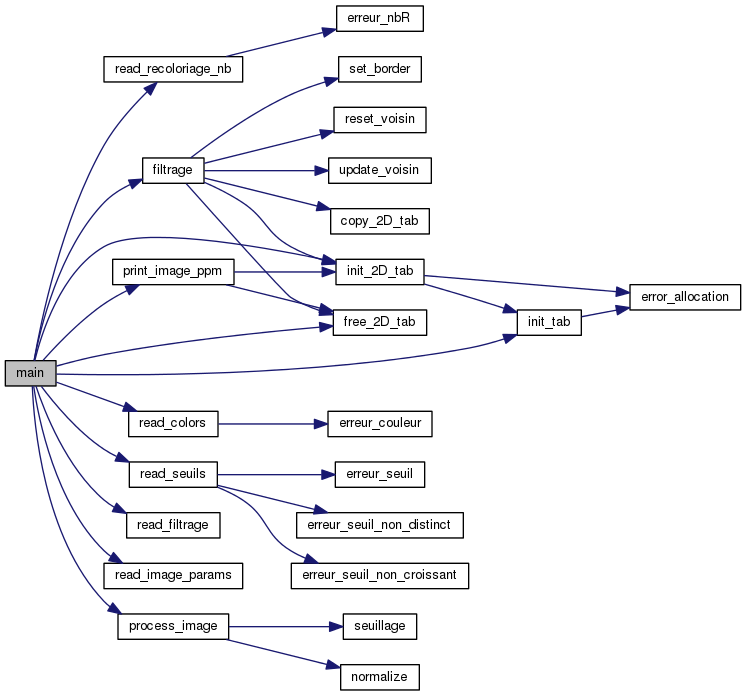
\includegraphics[scale=0.6]{graph.png}
\end{center}
\caption{Call graph}
\label{lastpage}
\end{figure}

\end{document}
